\special{pdf:minorversion 7}
\let\pdfcreationdate=\creationdate
\PassOptionsToPackage{dvipsnames}{xcolor}
\documentclass[12pt,letterpaper,twoside]{report}
%\usepackage{colorprofiles}
%\usepackage[a-2b,mathxmp]{pdfx}
\usepackage[todonotes={textsize=scriptsize}, final]{changes}
\usepackage[left=1in, right=1in, top=1in, bottom=1in]{geometry}
\usepackage{setspace}
\usepackage{layout}
\usepackage{parskip}
\usepackage{amsmath}
\usepackage{amssymb}
\usepackage[T1]{fontenc}
\usepackage{fontspec}
\setmainfont{XCharter}
\usepackage{unicode-math}
\setmathfont{XCharter-Math.otf}
\setsansfont{IBMPlexSans}[
    Extension = .otf,
    UprightFont = *-Regular,
    BoldFont = *-SemiBold,
    ItalicFont = *-Italic,
    BoldItalicFont = *-SemiBoldItalic,
    Scale = MatchLowercase
]
\setmonofont{IBMPlexMono}[Scale=MatchLowercase]
\usepackage{multicol}
\usepackage{multirow}
\usepackage{pdfpages}
\usepackage{pdflscape}
\usepackage{afterpage}
\usepackage{graphicx}
% \DeclareGraphicsExtensions{.png,.pdf}
\DeclareGraphicsExtensions{.pdf,.png}
\usepackage{tabularx}
% \usepackage{expl3}
% \usepackage{calc}
\usepackage[version=4]{mhchem}
\usepackage{siunitx}
\usepackage{bm}
\usepackage[dvipsnames]{xcolor}
\usepackage{caption}
\usepackage{subcaption}
\usepackage[sf,bf]{titlesec}
\usepackage{colortbl}
\usepackage{enumitem}
\usepackage{listings}
\usepackage{booktabs}
\usepackage{gensymb}
\usepackage[font=itshape]{quoting}
\usepackage{wrapfig}
\usepackage{fancyhdr}
\usepackage{lipsum}
\usepackage[final]{draftwatermark}
\usepackage{soul}
\usepackage[
    style=ieee,
    citestyle=numeric-comp,
    urldate=iso]{biblatex}
% \usepackage{datetime}
\usepackage{nameref}
\usepackage{hyperref}
\usepackage{tablefootnote}
\usepackage{todonotes}
\onehalfspacing
\definecolor{McGillRed}{cmyk}{0, 1, 0.9, 0}
\hypersetup{
    colorlinks=true,
    linkcolor=cyan,
    anchorcolor=cyan,
    citecolor=cyan,
    filecolor=cyan,
    urlcolor=cyan,
    pdftitle={Design and Validation of a Laser Thermal Propulsion Thruster Powered by a Fiber Laser},
    pdfauthor={Gabriel Roland Dubé},
    pdflang={en-CA},
    pdfsubject={For ambitious space missions like rapid human transit to Mars, conventional propulsion methods fall short. Laser-Thermal Propulsion (LTP) utilizes lasers to heat propellant gas, generating thrust with potentially greater specific impulse than traditional rocket engines. Two lab-scale LTP thrusters were tested in this thesis, denoted Version 1 (V1) and Version 2 (V2). Version 1 permitted initial testing and visualization of the Laser-Sustained Plasma (LSP) wave propagation. As a prototype for an actual thruster, Version 2 was optimized for thrust measurements. The design process of the improved V2 thruster is also presented. These thrusters were powered by a 300 W Continuous Wave (CW), 3 kW Quasi-Continuous Wave (QCW) 1.07 μm fiber laser. Argon was used as the propellant at a pressure of 20 bar, selected for its ease of ionization. Using an automotive-type coil, spark initiation of QCW LSP was successfully implemented in V1 and V2. Seeding of the argon with nitrogen dioxide (NO₂) at partial pressures between 0.12 bar to 0.55 bar showed the gas absorbed more than double the laser energy compared to pure argon propellant. To increase laser flux to the plasma, an optical system of two lenses was designed. Different lenses were compared using ray tracing software (WinLens3D). A CW LSP was achieved in V2, lasting 85.1 ms. This represents a 1.7 times longer lifetime than the maximum QCW pulse length of 50.0 ms at this power. Average cold flow thrust of V2 was approximately 1 N. In order to interpret the experimental results, a zero-dimensional (0D) heat transfer model was written in Python, using Bremsstrahlung as the mechanism of radiation. Finally, paths to further improve the V2 thruster and thrust stand are presented to eventually enable accurate thrust measurements with CW operation.},
    pdfkeywords={Laser thermal propulsion, Directed energy, Advanced propulsion, Interplanetary spaceflight, Space technologies},
    pdfstartview=
}
\setdeletedmarkup{\textcolor{McGillRed}{\sout{#1}}}
% \setdeletedmarkup{\textcolor{McGillRed}{#1}}
\definechangesauthor[color=violet, name={Emmanuel Duplay}]{ED}
\definechangesauthor[color=cyan, name={Barry Zandbergen}]{BZ}
\definechangesauthor[color=McGillRed, name={Andrew Higgins}]{AH}

\setlength{\marginparwidth}{2cm}

% \input{titlesec.tex}
\addbibresource{ref.bib}

\title{Laser-Powered Rocket Engine: small-scale experimental investigation}
\author{Gabriel Dubé}
\date{0000-00-00}

\renewcommand{\headrulewidth}{0pt}
\renewcommand{\chaptermark}[1]{\markboth{\MakeUppercase{\thechapter.\ #1}}{}}
\renewcommand{\sectionmark}[1]{\markright{\MakeUppercase{\thesection.\ #1}}}

\renewcommand{\chapterautorefname}{Chapter}
\renewcommand{\sectionautorefname}{Section}

\renewcommand\labelitemi{---}

\newcommand{\shotsettings}[4]{\texttt{#1}: #2~ms, \textit{f}/#3, ND#4}

\newcommand{\dd}[2]{\frac{\mathrm{d}#1}{\mathrm{d}#2}}
\newcommand{\ddi}[2]{\mathrm{d}#1/\mathrm{d}#2}

\newcommand{\blankpage}{%
    \null
    \thispagestyle{empty}%
    \addtocounter{page}{-1}%
    \newpage}

% Track changes commands
% \newcommand{\change}[1]{\textcolor{McGillRed}{#1}}
% \newenvironment{changeblock}{\color{McGillRed}}{}
% \renewcommand{\change}[1]{#1}  % Comment out to suppress changes
% \renewenvironment{changeblock}{}{}  % Comment out to suppress changes

\fancypagestyle{fancy}{
    \fancyhf{}
    \fancyhfinit{\sffamily}
    \lhead{\leftmark}
    \rhead{\rightmark}
    % \lfoot{AE5050}
    % \rfoot{\thepage}
    \fancyfoot[LE,RO]{\thepage}
    %\fancyfoot[RE,LO]{AE5050}
}

\fancypagestyle{plain}{
    \fancyhf{}
    \fancyfoot[C]{\sffamily \thepage}
    
}

\pagestyle{fancy}

\SetWatermarkText{\sffamily \textbf{DRAFT}}
\SetWatermarkFontSize{2cm}
\SetWatermarkColor[gray]{0.85}
    
\input{lstStyle.tex}
\input{customenvs.tex}

\sisetup{detect-all}

\begin{document}
    \setlength{\parindent}{0pt}
    \setlength{\headheight}{27.4pt}
    % \includepdf{assets/cover.pdf}
    \begin{titlepage}
  \thispagestyle{empty}
  \sffamily
  \begin{center}
    \includegraphics[width=0.5\textwidth]{assets/McGill_logo.pdf} \\
    \vspace*{2cm}
    
    \huge
    \textbf{Design and validation of an Argon Laser Thermal Propulsion Thruster Powered by a Fiber Laser}
    
    \large
    % \textit{Small-scale experimental investigation}     

    
    \vspace{1.5cm}    
    \textbf{Gabriel Roland Dubé}\\

    
    \vspace{0.5cm}
    Department of Mechanical Engineering\\
    McGill University, Montreal\\

    \vspace{1.5cm}
    December 2024\\
    \vspace{1.5cm}
    
    A thesis submitted to McGill University \\
    in partial fulfillment of the requirements of the degree of\\
    \textbf{Master of Science}\\
    
    %\vskip 10mm
    \vfill

    {\color{red}\hrule}

    \copyright Gabriel Roland Dubé, 2024
            
  \end{center}
\end{titlepage}

    \pagenumbering{roman}
    
    
    \hypersetup{linkcolor=black}
    \tableofcontents
    
    \listoffigures
    \addcontentsline{toc}{chapter}{List of Figures}
    
    \listoftables
    \addcontentsline{toc}{chapter}{List of Tables}
    \hypersetup{linkcolor=cyan}
    
    \input{chapters/0_1_nomenclature.tex}

    % ------------  UNCOMMENT THESE!!!! ------------------

    \newpage
    \begin{plainchp}{Abstract}
    \addcontentsline{toc}{chapter}{Abstract}
    
    For ambitious space missions like rapid human transit to Mars, conventional propulsion methods fall short. Laser-Thermal Propulsion (LTP) utilizes lasers to heat propellant gas, generating thrust with potentially greater specific impulse than traditional rocket engines. Two lab-scale LTP thrusters were tested in this thesis, denoted Version 1 (V1) and Version 2 (V2). Version 1 permitted initial testing and visualization of the Laser-Sustained Plasma (LSP) wave propagation. As a prototype for an actual thruster, Version 2 was optimized for thrust measurements. The design process of the improved V2 thruster is also presented. These thrusters will both be powered by a \qty{300}{W} Continuous Wave (CW), \qty{3}{kW} Quasi-Continuous Wave (QCW) \qty{1.07}{μm} fiber laser. Argon was used as the propellant at a pressure of \qty{20}{bar}, selected for its ease of ionization. Using an automotive type coil, spark initiation of QCW LSP was successfully implemented in V1 and V2. Seeding of the argon with nitrogen dioxide (\ce{NO2}) at partial pressures between \qtyrange{.12}{.55}{bar} showed the gas absorbed more than double the laser energy compared to pure argon propellant. To increase laser flux to the plasma, an optical system of two lenses was designed. Different lenses were compared using ray tracing software (WinLens3D). A CW LSP was achieved in V2, lasting \qty{85.1}{ms}. This represents a 1.7 times longer lifetime than the maximum QCW pulse length of \qty{50.0}{ms} at this power. Average cold flow thrust of V2 was \qty{0.96}{N}. In order to interpret the experimental results, a zero-dimensional (0D) heat transfer model was written in Python, using Bremsstrahlung as the mechanism of radiation. Finally, paths to further improve the V2 thruster and thrust stand are presented to eventually enable a CW hot fire test.

\end{plainchp}
    % LTeX: language=fr

\begin{plainchp}{Résumé}
    \addcontentsline{toc}{chapter}{Résumé}

    La propulsion laser-thermique (LTP) utilise des lasers pour chauffer le gaz propulseur, générant ainsi de la poussée avec une impulsion spécifique potentiellement plus grande que les moteurs fusées traditionnels. Dans cette thèse, deux propulseurs LTP à l'échelle du laboratoire ont été testés : Version 1 (V1) et Version 2 (V2). Le processus de conception du propulseur amélioré V2 est également présenté. Ces deux propulseurs seront alimentés par un laser à fibre de \qty{1.07}{μm} ayant une puissance ondes continues (CW) de \qty{300}{W} et une puissance à ondes quasi continues (QCW) de \qty{3}{kW}. L'argon est utilisé comme gaz propulseur à une pression de \qty{20}{bar}. L'amorçage par étincelle du plasma soutenu par laser (LSP) QCW a été implémenté avec succès dans V1 et V2. L'ensemencement en \ce{NO2} de l'argon à des pressions partielles comprises entre \qtyrange{.12}{.55}{bar} a montré que le gaz absorbait plus du double de l'énergie laser par rapport à de l'argon pur. Pour augmenter le flux laser vers le plasma, un système optique composé de deux lentilles a été conçu. Un LSP CW a été obtenu avec V2, d'une durée de \qty{85.1}{ms}. Cela représente une durée de vie 1.7 fois plus longue que la longueur d'impulsion QCW maximale de \qty{50.0}{ms} à cette puissance. La poussée moyenne à froid de V2 était de \qty{0.96}{N}. Afin d'interpréter les résultats expérimentaux, un modèle de transfert de chaleur zéro dimension (0D) a été écrit en Python, en utilisant le Bremsstrahlung comme mécanisme de rayonnement. Enfin, des pièces permettant d'améliorer le propulseur V2 sont présentées pour éventuellement permettre un essai CW à chaud du propulseur.
    
\end{plainchp}
    \begin{plainchp}{Acknowledgements}
    \addcontentsline{toc}{chapter}{Acknowledgements}
    
    First, I want to thank my supervisor, Professor Andrew J. Higgins, for his deep knowledge, mentorship and support throughout this journey. He gave me and our lab the singular opportunity to pursue graduate studies on advanced space propulsion. In Canada, this is a rare topic of research indeed, but it is only with advances in this field that humanity will be able to reach the stars.

    Thank you to my family for their support and encouragement during my studies.

    I would like to extend my heartfelt appreciation to the members of the McGill Interstellar Flight Experimental Research Group. Emmanuel and Siera, in the pursuit of science together, you have given me dear memories that will last a lifetime. I wish Siera and Anthony much success in continuing the work Emmanuel and I have but started.

    Editorial help was provided by Emmanuel Duplay, Siera Riel, John Kokkalis, Sebastian Rodriguez, and Dan-Cornelius Savu. Sebastian helped manufacture the V2 electrodes. Thank you for your knowledge on how to do things in the lab. Thariq Meulendijks did the needle valve $A^*$ calibration and led the bubble flow meter experiments.

    Alain Halbouny, Jade Tabbara, Karl Atallah, Serge Rubeiz, and Shady Tawil designed and assembled the Version 2 (V2) laser-thermal thruster, as well as produced its drawings and renders. Thank you to Meisam Aghajani, Mathieu Beauchesne, Ramnarine Harihar (Harry), and Andy Hofmann, the machinists who built V2. Without it, we would not have the experimental insights we have today.

    This work was funded by the Natural Sciences and Engineering Research Council of Canada (NSERC) Canada Graduate Scholarships — Master's (CGS-M) program and the McGill Summer Undergraduate Research in Engineering (SURE) program.

\end{plainchp}
    \afterpage{\blankpage}
    \newpage
    \pagenumbering{arabic}

    % \input{chapters/unnumberedchapter.tex}

    %UNCOMMENT THESE!!!!
    
    \chapter{Introduction} \label{chp:intro}
% \addcontentsline{toc}{chapter}{Unnumbered Chapter}  % Uncomment to include in ToC
% \markboth{\MakeUppercase{Unnumbered Chapter}}{}

    \setcounter{chapter}{2}
\chapter{Facility design}

    \section{Version 1 test section} \label{sec:design_v1}

        The design process of the first generation thruster, called Version 1 (V1, see \autoref{fig:V1 setup}), can be found in \textcite{duplayArgonLaserPlasmaThruster2024a}. It proved to be a dependable prototype, repurposed from a previous unrelated experiment. However, it presented problems that required a second generation prototype to be designed and manufactured.

        \begin{figure}[!ht]
            \centering
            \begin{subfigure}[t]{\textwidth}
                \centering
                \includegraphics[width=0.85\textwidth]{assets/3 design/finalsetup_static.pdf}
                \caption{Static setup}
            \end{subfigure}
            \hfill
            \begin{subfigure}[t]{\textwidth}
                \centering
                \includegraphics[width=0.85\textwidth]{assets/3 design/finalsetup_flowing.pdf}
                \caption{Flowing setup}
            \end{subfigure}
            \caption{V1 LTP thruster from \textcite{duplayArgonLaserPlasmaThruster2024a}}
            \label{fig:V1 setup}
        \end{figure}

        298 recorded pulsed laser shots were conducted with V1, exploring the power-pressure threshold, wire initiation and spark initiation. A side window permitted direct visualization of the LSP with a high speed camera (Photron Fastcam SA5).

    \section{Version 2} \label{sec:design_v2}

        To improve upon the V1 facility, an entire LTP thruster redesign was done. This resulted in the much smaller Version 2 (V2) purpose-built LTP thruster at the end of April 2024, seen in \autoref{fig:V2 render}.

        \begin{figure}[!ht]
            \centering
            \begin{subfigure}[t]{\textwidth}
                \centering
                \includegraphics[width=0.85\textwidth]{assets/3 design/V2 render 45 view.png}
                \caption{View of the laser path (in red) and thruster mounted on its thrust stand}
            \end{subfigure}
            \hfill
            \begin{subfigure}[t]{\textwidth}
                \centering
                \includegraphics[width=0.85\textwidth]{assets/3 design/V2 render cutout.png}
                \caption{Cutaway view of the inside of the thruster}
            \end{subfigure}
            \caption{Render of the V2 LTP thruster}
            \label{fig:V2 render}
        \end{figure}

        \subsection{Requirements}

            The following requirements were developed for the design of the V2 thruster. The objective was to detect a measurable difference in thrust between an argon cold gas thruster and an argon “hot gas” thruster, heated by a laser supported plasma (LSP).

            \begin{enumerate}
                \item Laser thruster
                \begin{enumerate}
                    \item A \qty{300}{W} Continuous Wave (CW) \qty{1070}{nm} laser shall sustain the plasma (Nominal power \qty{300}{W}, actual max power \qty{350}{W})
                    \item The thruster shall have a minimum safe “hot” operation time of \qty{30}{s}
                    \begin{enumerate}
                        \item In the event of failed LSP initiation, the thruster shall safely absorb the total laser power for at least \qty{10}{s}
                    \end{enumerate}
                    \item An optical path shall be present to let the laser into the thruster, utilizing a \qty{100}{mm} focal length lens at minimum and a collimated beam with a maximum diameter of \qty{30}{mm}
                    \begin{enumerate}
                        \item The optical components shall not be damaged by the laser flux
                    \end{enumerate}
                    \item Argon shall be used as the working fluid
                    \begin{enumerate}
                        \item The argon feed gas shall be at room temperature
                    \end{enumerate}
                    \item A gas feed path shall bring argon gas into the thruster
                    \begin{enumerate}
                        \item The gas feed shall be choked at the thruster inlet
                        \item The gas feed shall be evenly distributed in the thruster
                    \end{enumerate}
                    \item The mass flow rate of the argon gas shall be measured and controlled by interchangeable upstream choked orifices
                    \item The maximum allowable operating pressure (MAOP) of the thruster shall be 50 bar
                    \begin{enumerate}
                        \item The nominal pressure of the thruster shall be 25 bar
                    \end{enumerate}
                    \item A converging-diverging exhaust nozzle shall be designed to accelerate the gas to a supersonic speed
                    \begin{enumerate}
                        \item The nozzle shall be easily changeable
                    \end{enumerate}
                    \item A 1/8" NPT port for a pressure transducer shall be present along the thruster
                    \item An optical port shall be present for spectrometry measurements of the plasma
                    \item The thruster shall be installed on a thrust stand (See requirements section 3. Thrust stand)
                \end{enumerate}
                \item Initiation system/electrical
                \begin{enumerate}
                    \item The LSP shall be initiated by an electrical spark
                    \item The spark gap shall be measurable, controllable, and repeatable
                    \item The spark shall be generated by an AEM 30-2853 High Output Smart Coil, supplying \qty{41}{kV} with up to \qty{118}{mJ}
                    \item All parts of the thruster and thrust stand shall be directly or indirectly connected to a common electrical ground
                \end{enumerate}
                \item Thrust stand
                \begin{enumerate}
                    \item The thrust stand shall measure thrust on the order of \qtyrange{0.1}{5}{N}
                    \item The thrust stand shall minimize friction losses
                    \item The thrust stand shall be securely fixed using standard optical breadboard mounting hardware
                \end{enumerate}
            \end{enumerate}

            With these requirements, preliminary geometric dimensions of the V2 thruster could commence. It was expected to be much smaller than V1, as the goal was to isolate the LSP region and increase heat flux to the gas.

        \subsection{Initial sizing of the double choked LTP thruster}

            The minimum diameter of the cylinder that will contain the LSP core must be larger than the diameter of the plasma itself, which is \qty{2}{mm} according to observations from \textcite{duplayArgonLaserPlasmaThruster2024a}. An arbitrary factor of safety of 2.5 was used, which set the innermost diameter to \qty{5}{mm}.

            The argon gas enters radially near the end of the thruster. A channel around the inner cylinder directs the gas to the front of the thruster, where it turns \qty{180}{\degree} through the plasma region and out the nozzle (see \autoref{fig:double choke sizing}). This ``cylinder-inside-a-cylinder" design was inspired by \textcite{toyodaThrustPerformanceCW2002}, allowing the gas to cool the inner cylinder and straightening the flow.

            The thickness of the exterior wall of the thruster was determined by the minimum engagement depth (\qty{14}{mm}) of the 1/4 inch Ultra-Torr NPT fittings.

            The required metering valve and nozzle orifice sizes were then estimated. When adding energy to the thruster chamber with a laser, it is useful to choke the inflow upstream of the chamber. Indeed, this keeps the $P_0$ and $\dot{m}_\mathrm{in}$ constant, so the increase in chamber pressure can be interpreted as a measure of energy deposition. The second choke happens at the nozzle to accelerate the hot gas to a supersonic speed. Therefore, this configuration is double choked (see \autoref{fig:double choke sizing}), a classic problem in compressible fluid mechanics.

            \begin{figure}[h]
                \centering
                \includegraphics[width=0.8\linewidth]{assets/3 design/Double choked LTP thruster.pdf}
                \caption{Cutaway of the V2 double choked LTP thruster showing both choking orifices: the metering valve and the nozzle. Ports other than the argon inlet are omitted for clarity.}
                \label{fig:double choke sizing}
            \end{figure}
            
            The starting assumptions were the following: a \qty{300}{W} power input (the laser) supplies energy to an LTP experiment that has an internal pressure of \qty{25}{bar}, with a \qty{50}{bar} feed pressure. It is required that the hot gas operation (laser on) increases the gas' exit velocity to twice that of the cold gas operation (laser off). The gas mass flow rate and the diameter of the two orifices needed to choke the flow will be determined.

            Starting with a cold gas thruster using argon, the speed of sound of argon ($c_0$) is \qty{323}{m/s}. This is at ambient temperature (\qty{300}{K}), as we have no laser energy to heat the gas in this case. With a nozzle, the gas is accelerated to approximately twice this speed. The exit velocity of the gas $v_\mathrm{exit}$, which is our main performance parameter, is therefore \qty{646}{m/s}.
            
            Laser on (hot) operation will now be examined. Taking the previous $v_\mathrm{exit}$ and ionizing the whole flow, it is assumed that the thruster's efficiency is doubled. This gives a $v_\mathrm{exit}\approx \qty{1300}{m/s}$. What nozzle throat size is therefore necessary for this $\dot m$ with $p_\mathrm{chamber} = \qty{25}{bar}$? $\mathrm{MW_{Ar}} = \qty{40}{g/mol}$ and the speed of sound is $c = \sqrt{\gamma R T}$. As the speed of sound will be doubled, the temperature is multiplied by 4.
            \[\text{Power} = \dot m (h_2-h_1)
            = \dot m c_p (T_2-T_1)\]
            Using a constant $c_p$ of argon of \qty{0.520}{kJ.kg^{-1}.K^{-1}}, the calculated $\dot m$ is \qty{0.641}{g/s}. Fliegner's formula describes the mass flow rate of an isentropic flow:
            \[\frac{\dot m}{A} = p_0\sqrt{\frac{\gamma}{T_0 R}}\frac{M}{(1+\frac{\gamma-1}{2}M^2)^{(\frac{\gamma+1}{2(\gamma-1)})}}\]
            With $\gamma = \frac{c_p}{c_v} = 1.67$ for argon and choked flow at the nozzle, the area and the diameter of the circular nozzle are \qty{0.176}{mm^2} and \qty{0.473}{mm}, respectively. The V2 test section was built with this nozzle diameter. These calculations can be repeated for the feed orifice, with the same $\dot m$, a pressure of \qty{50}{bar} and ambient temperature. This gives us an orifice diameter of about 0.2 mm.
        
        \subsection{Test section and thrust stand}
            
            As can be seen in \autoref{fig:V2 setup}, the V2 test section was designed with multiple ports for modularity, enabling static and flowing tests with argon propellant. Ports that were not in use were fitted with pipe plugs. In all tests, the two opposing electrode ports and one argon inlet port were used. The second argon inlet, intended to offer a more uniform flow if needed, was not used. The optical access port was initially fitted with a quartz rod in an Ultra-Torr fitting, but was replaced by a pipe plug after excessive rod breakage. After flowing through the test section, used argon propellant was vented to the ambient air. \autoref{fig:V2 IRL setup} shows the two final configurations that were used.

            \begin{figure}[!ht]
                \centering
                \begin{subfigure}[t]{\textwidth}
                    \centering
                    \includegraphics[width=0.85\textwidth]{assets/3 design/V2 Static config.pdf}
                    \caption{Static configuration}
                \end{subfigure}
                \hfill
                \begin{subfigure}[t]{\textwidth}
                    \centering
                    \includegraphics[width=0.85\textwidth]{assets/3 design/V2 Flowing config.pdf}
                    \caption{Flowing configuration}
                \end{subfigure}
                \caption{V2 LTP thruster}
                \label{fig:V2 setup}
            \end{figure}

            \begin{figure}[!ht]
                \centering
                \begin{subfigure}[t]{0.45\textwidth}
                    \centering
                    \includegraphics[width=\textwidth]{assets/3 design/V2 Static configuration.jpg}
                    \caption{Final static configuration. Note the extension part and window mount. Optics and laser collimator are not pictured here, but would be installed during testing.}
                \end{subfigure}
                \hfill
                \begin{subfigure}[t]{0.45\textwidth}
                    \centering
                    \includegraphics[width=\textwidth]{assets/3 design/V2 flowing setup.jpg}
                    \caption{Final flowing configuration. The nozzle is held by the rear plate.}
                \end{subfigure}
                \caption{V2 LTP thruster}
                \label{fig:V2 IRL setup}
            \end{figure}

            The thrust stand is a ball bearing carriage (McMaster-Carr 6709K12) on a \qty{15}{mm} wide, \qty{160}{mm} long guide rail (McMaster-Carr 6709K33). The rail is mounted on the optical breadboard using acrylic spacers. A string through a pulley holds a variable weight, adding a preload to the test section. This ensures adequate contact between the test section and the load cell, and allows calibration of the load cell. Two load cells are used with different force sensing range: Honeywell FSG020WNPB (\qtyrange{0}{20}{N}) and Honeywell FSG005WNPB (\qtyrange{0}{5}{N}).

        \subsection{Laser and optics}

            The laser used as the plasma's power source is an IPG Photonics YLR-300/3000-QCW-MM-AC Ytterbium fiber laser. The wavelength of the emitted light is \qty{1070}{nm}. Its nominal maximum power is \qty{3}{kW} quasi-continuous wave (QCW) or \qty{300}{W} continuous wave (CW). At \qty{3}{kW}, a QCW pulse has a maximum duration of \qty{10}{ms}. The maximum duration of a \qty{300}{W} QCW pulse is \qty{50}{ms}. The IPG Photonics P30-001736 collimator outputs a \qty{30}{mm} diameter laser beam. The laser also includes a red visible laser for alignment, which is coaxial to the main beam. These components form the laser system, presented in \autoref{fig:laser and collimator}.

            \begin{figure}[!ht]
                \centering
                \begin{subfigure}[t]{0.45\textwidth}
                    \centering
                    \includegraphics[width=\textwidth]{assets/3 design/Laser box.jpg}
                    \caption{IPG Photonics YLR-300/3000-QCW-MM-AC laser}
                \end{subfigure}
                \hfill
                \begin{subfigure}[t]{0.45\textwidth}
                    \centering
                    \includegraphics[width=\textwidth]{assets/3 design/Laser aperture.jpg}
                    \caption{IPG Photonics P30-001736 collimator}
                \end{subfigure}
                \caption{Laser system}
                \label{fig:laser and collimator}
            \end{figure}

            Calibration reports for the laser and the collimator can be found in \autoref{chp:app_YLR}. The laser is mounted at the base of a freestanding electronics rack (\autoref{fig:electronics rack}).

            \begin{figure}[!ht]
                \centering
                \includegraphics[width=0.50\textwidth]{assets/3 design/Control rack.jpg}
                \caption{Electronics rack with laser at the base}
                \label{fig:electronics rack}
            \end{figure}

            V2 uses two lenses placed close to each other to focus the laser from the collimator. These are the Thorlabs LA1380-C and LA1417-C N-BK7 plano-convex lenses with a \qtyrange{1050}{1700}{nm} anti-reflective coating. Their focal lengths of \qty{500}{mm} and \qty{150}{mm}, respectively, give a combined focal length of \qty{115}{mm}. These two lenses are mounted in a single Thorlabs LMR2 lens mount with two retaining rings. A Thorlabs DT12 translation stage enables left/right alignment of the laser focus, while a Thorlabs DTS25 translation stage gives control on the depth (axial position) of the focus.

        \subsection{Timing control}

            Correct timing of the laser and spark initiation is necessary to initiate LSP. To this end, delay generators are used (BNC models 7010 and 7055) as seen in \autoref{fig:timing section and oscilloscope}. They are mounted at the top of the electronics rack.

            \begin{figure}[!ht]
                \centering
                \includegraphics[width=0.50\textwidth]{assets/3 design/Timing rack and oscilloscope.jpg}
                \caption{Delay generators and oscilloscope}
                \label{fig:timing section and oscilloscope}
            \end{figure} 

        \subsection{Data acquisition (DAQ) system and oscilloscope}

            Load cell and pressure transducer voltage is sent to a DATAQ Instruments DI-2018, on \autoref{fig:DAQ}. This data is streamed to a personal computer by USB, where the thrust and pressure traces can be saved for analysis. Two pressure sensors were used: a PCB Model 113B28 and an Omega PX119A-1KG5V. Refer to \autoref{chp:omega calibration} for the Omega pressure sensor calibration.

            \begin{figure}[!ht]
                \centering
                \includegraphics[width=0.50\textwidth]{assets/3 design/DAQ electronics.jpg}
                \caption{DAQ system}
                \label{fig:DAQ}
            \end{figure}

        \subsection{Cameras}

            A Photron SA5 high speed camera was used during certain LSP shots to determine if LSP initiation had happened and how long the plasma had lasted. Due to no side windows being present on V2, the Photron camera looked at an angle from the side into the front window, seeing the reflection of the plasma core (as in \autoref{fig:V2 setup}). During LSP shots, the camera's lenses and its sensor were protected by an Aurora PowerXND-II Variable Neutral Density Filter and a Hoya \qty{58}{mm} UV and IR cut filter.

            A generic USB webcam was also connected to the data acquisition laptop, giving a live wide-angle view of the entire experiment. As these cameras are sensitive to IR, it gave an additional confirmation that the laser emission was turned off before opening the laser safety curtain.

        \subsection{Spark initiation system}

            The spark was generated by an AEM 30-2853 High Output Smart Coil, supplied by a \qty{10}{A} power supply. The coil can generate a \qty{40}{kV}, \qty{103}{mJ} spark. The trigger signal wire from the delay generator comes in from the left of \autoref{fig:Spark initiation}. It passes through the power supply electrical box in a quad shielded coaxial cable. The smart coil is placed in a separate electrical box to reduce electromagnetic interference. The spark energy exits through the cable on the right of \autoref{fig:Spark initiation}. 

            \begin{figure}[!ht]
                \centering
                \includegraphics[width=0.50\textwidth]{assets/3 design/Spark initiation system.jpg}
                \caption{Spark initiation system. On the left is a power supply, while spark coil number 6 is on the right.}
                \label{fig:Spark initiation}
            \end{figure}

            \autoref{fig:Assembled electrode design} shows the assembled electrodes, the sharper one being connected to the smart coil's output. The other electrode is grounded.

            \begin{figure}[!ht]
                \centering
                \includegraphics[width=0.5\textwidth]{assets/3 design/V2 electrodes.jpg}
                \caption{Assembled electrodes with Ultra-Torr cap and electrical connectors}
                \label{fig:Assembled electrode design}
            \end{figure}

        \subsection{Needle valve}
            
            To be able to run the thruster in the double choked configuration, an adjustable orifice upstream of the thruster is required. The WL14H-320P needle valve (\autoref{fig:Needle valve}) was chosen for this.

            \begin{figure}[!ht]
                \centering
                \includegraphics[width=0.50\textwidth]{assets/3 design/Needle valve.jpg}
                \caption{WL14H-320P Needle valve}
                \label{fig:Needle valve}
            \end{figure}

        \begin{figure}[!ht]
            \centering
            \includegraphics[width=\textwidth]{assets/3 design/V1 V2 comparison.png}
            \caption{Size comparison between V1 (top, on extrusion rails) and V2 (bottom, mounted in front of laser collimator). V2 is in static configuration, without the extension cylinder.}
        \end{figure} 
    \chapter{Experiments}

    The following chapter will explain the methodology and the results of the various experiments undertaken to validate and characterise the V2 thruster.

    \section{Static LSP validation}


    \section{Cold flow thruster characterisation}

        \subsection{Cold flow thrust tests}

        \subsection{Thruster nozzle effective sonic area $A^*$}

            To characterise the effective sonic area, $A^*$, of the thruster nozzle, a choked orifice blow-down test was undertaken based upon the theory in \textcite{saadCompressibleFluidFlow}. V2 in flowing configuration was pressurized to \qty{20}{bar}. The argon flow was then closed. The pressure curve was recorded by the Omega \todo{part number} transducer.
            
            \missingfigure{blowdown pressure curve}


            \todo{In discussion, talk about the issue of A* with 5 papers from June 4th on slack.}

            The following expression for a pressure-time history \todo{change this wording} was then implemented in Python:

            \[
            
            \]

            The best match was found to be a diameter of \qty{0.23}{mm}.



        \subsection{Needle valve effective sonic area $A^*$}

        \subsection{Mass flow rate $\dot m$}

            [TODO: add experiment with me and Tariq]

        \subsection{Summary of results}

            The following table presents a summary of the results determined from cold flow thruster characterisation.

            \begin{table}[!ht]
                \caption{Summary of the studied V2 thruster characteristics}
                \label{tab:characteristics}
                \begin{tabularx}{\textwidth}{XX}
                Characteristic             & Value and unit \\
                mdot                       &                \\
                Valve A*                   &                \\
                Nozzle A*                  &                \\
                Internal volume of thruster in flowing configuration        &                \\
                Cold flow thrust at 20 bar &               
                \end{tabularx}
            \end{table}

    % OLD TEXT OLD TEXT --------------------------------------------
    \section{ANYTHING AFTER THIS IS OLD TEXT}

    \section{V1 experiments}
        
        Spark ignition shots

    \section{V2 experiments}
        This section presents the various experiments that were conducted with the V2 thruster, as well as improvements that were made to this thruster while operating it.
    
        \subsection{Initial LSP shots}

            With the Photron SA5 looking into the thruster from the front, LSP initiation was confirmed in V2.

            % put this in discussion
            \begin{figure}[!ht]
                \centering
                \includegraphics[width=0.75\textwidth]{assets/4 experiments/V2 test damage.jpg}
                \caption{Damage to the thruster after two \qty{3}{kW} laser shots}
            \end{figure}

            \begin{figure}[!ht]
                \centering
                \includegraphics[width=0.75\textwidth]{assets/4 experiments/V2 test damage.jpg}
                \caption{Damage to the thruster after two \qty{3}{kW} laser shots}
            \end{figure}

            % Stills of first High-speed LSP video, showing expansion of LSP wave like in V1

            As these are at an angle and we are looking at the reflection of the LSP, no LSP velocity measurements can be made.
        
        \subsection{Cold flow thrust tests}

            Cold flow tests were completed to give a baseline measurement of thrust before hot fire tests, and to validate the functioning of all data acquisition systems.
            
            % thrust vs pressure graph

            
        
        \subsection{Effective throat area}
            
            With the cold flow thrust tests completed, the effective throat area, $A^*$, was determined. Although the throat was machined to be \qty{0.7}{mm} in diameter, boundary layer effects at this size greatly reduce the effective throat area.

            [ADD SAAD BLOWDOWN DISCUSSION]

            [CITE 2 ASME STUDIES]


        \subsection{First CW LSP}
            
            A \qty{100}{\%} power CW shot was then attempted at \qty{20}{bar} argon. 

            [photo of laser on, Spark/LSP initiation, LSP constant, laser off (LSP dying down)]

            First the laser is turned on. A flash marks the spark initiation and instant LSP initiation. The CW LSP was kept running for about a second before the laser turns off and the LSP dies down.

            \begin{figure}[!ht]
                \centering
                \includegraphics[width=0.5\textwidth]{assets/4 experiments/CW pressure rise.png}
                \caption{Pressure rise with PCB transducer}
            \end{figure}

            This graph shows the pressure rise recorded by the PCB transducer connected to the oscilloscope. As it is a dynamic sensor, this graph has little value, although it is included as a result to support CW LSP initiation. This was the first CW LSP generated in the lab. Minimal damage to the window was noticed after this test, showing that the LSP absorbs a significant amount of energy.

        \subsection{Window extension tube}
            
            After the first CW LSP, more CW and pulsed shots were attempted. These continued to damage the rear window. Eventually, a \qty{3}{s} CW shot melted it severely enough that 

            \begin{figure}[!ht]
                \centering
                \includegraphics[width=0.5\textwidth]{assets/4 experiments/window damage.jpg}
                \caption{Rear window damage on V2}
            \end{figure}

            The solution chosen was to manufacture a window extension tube, moving the rear window downstream to where the laser flux density is comparable to the front window, where no damage was seen.

            [drawing of extension tube]


        


        % \subsection{CW LSP (hot fire) thrust tests}

        %     Find m dot, show thrust graph. Get Isp from these. Compare to other thrusters in the literature. Get heat deposition efficiency somehow? Or use Toyoda's definition of efficiency that only uses power in.

        \section{Summary of results}

            \begin{table}[]
                \caption{Summary of the studied V2 thruster characteristics}
                \label{tab:characteristics}
                \begin{tabular}{ll}
                Characteristic             & Value and unit \\
                mdot                       &                \\
                Valve A*                   &                \\
                Nozzle A*                  &                \\
                Internal volume            &                \\
                Cold flow thrust at 20 bar &               
                \end{tabular}
            \end{table}
 

            

        




    \chapter{0D LSP Model} \label{chp:models}

    To predict experimental data, namely the pressure increase of the gas that should be expected when laser energy is input, the heat capacity of argon and hydrogen was modelled. A zero-dimensional (0D) heat transfer model was then written in Python to compare to experimental data. Argon and hydrogen were used to validate initial equilibrium calculations, while the 0D model was solely implemented using argon. Argon is the current gas used in experiments, as it is economical and easy to ionize. Hydrogen is projected to be used in a full-scale LTP engine for its increased $I_\mathrm{sp}$ due to its lower molecular weight.

    \section{Equilibrium calculations} \label{sec:equilibrium calcs}
        
        The following seventh order polynomials and their coefficients ($a_1$ to $a_7$, $b_1$, and $b_2$), from \textcite{mcbrideNASAGlennCoefficients2002}, were implemented in Python. Species of interest were \ce{H}, \ce{H2}, \ce{Ar}, \ce{Ar+}, and electrons \ce{e-}. Plasma temperatures studied allowed us to treat the argon as singly ionized, and the hydrogen as dissociated. The heat capacity at constant pressure, as well as the temperature ($T$) dependent part of enthalpy and entropy of each species are given by $c_p^0$, $h^0$ and $s^0$, respectively. $\bar R$ is the universal gas constant.

        \begin{equation}
            c_p^0 (T)/\bar R = a_1 T^{-2} + a_2 T^{-1} + a_3 + a_4   T + a_5 T^2 + a_6 T^3 + a_7 T^4
        \end{equation} 
        
        \begin{equation}
            h^0 (T)/\bar RT = -a_1 T^{-2} + a_2 \ln(T)/T + a_3 + a_4 T / 2 + a_5 {T^2}/3 + a_6 {T^3}/4 + a_7 {T^4}/5 + b_1/T
        \end{equation}
        
        \begin{equation}
            s^0(T)/\bar R = -a_1 T^{-2}/2 - a_2 T^{-1} + a_3\ln(T) + a_4   T + a_5 {T^2}/2 + a_6 T^3/3 + a_7 T^4/4 + b_2
        \end{equation}

        Next, the functions for entropy $\bar s_i$ of each species $i$ and Gibbs energy $\bar g_i$, both per \unit{kmol}, were implemented. These values depend on temperature $T$ and partial pressure $p_i$. $y_i$ is the molar fraction of the species, and $p_\mathrm{ref}$ is the reference pressure, equal to \qty{1}{bar}.
        
        \begin{equation}
            \bar s_i (T, p_i) = \bar s_i^0 (T) - \bar R \ln \frac{y_i p}{p_\mathrm{ref}}
        \end{equation}

        \begin{equation}
            \bar g_i = \bar h_i - T \bar s_i
        \end{equation}

        Considering the number of moles $n_i$, expressions of the Gibbs energy of the two mixtures $G_\mathrm{mixture}$ are found:

        Starting with \qty{1}{kmol} argon,
        \begin{equation}
            G_\mathrm{mixture,\: Ar}(T, p) = n_\mathrm{Ar} \bar g_\mathrm{Ar}(T, p_\mathrm{Ar}) + n_\mathrm{Ar+} \bar g_\mathrm{Ar+}(T, p_\mathrm{Ar+}) + n_\mathrm{e} \bar g_\mathrm{e}(T, p_\mathrm{e})
        \end{equation}

        Starting with \qty{1}{kmol} hydrogen,
        \begin{equation}
            G_\mathrm{mixture,\: H_2}(T, p) = n_\mathrm{H} \bar g_\mathrm{H}(T, p_H) + n_\mathrm{H2} \bar g_\mathrm{H2}(T, p_\mathrm{H2})
        \end{equation}

        \autoref{fig:Gibbs} plots the Gibbs energy of the hydrogen mixture as a function of its degree of dissociation $x$, for different total pressures $p$.

        \begin{figure}[!ht]
            \centering
            \includegraphics[width=0.7\textwidth]{assets/2 models/Gibbs.pdf}
            \caption{Gibbs free energy (G) plotted against the degree of dissociation (x) of hydrogen under three different pressures}
            \label{fig:Gibbs}
        \end{figure}

        A similar dissociation graph can be found with argon, but with three species. The Gibbs energy is then minimized to determine the molar fractions $y_i$ at which the mixture reaches equilibrium. From this, the enthalpy $H$ of the mixture was found. The $C_p$ of the mixture was then calculated from the enthalpy with:

        \begin{equation}
            C_p = \frac{\partial H}{\partial T}\bigg|_{p = const.}
        \end{equation}
        
        For argon, these calculated $C_p$ values were validated against values from CEA \cite{CEARUNRev4} in \autoref{fig:Cp_compare}.
        
        \begin{figure}[!ht]
            \centering
            \includegraphics[width=0.7\textwidth]{assets/2 models/Cp_compare.pdf}
            \caption{Comparing calculated $C_p$ values of argon to those from CEA}
            \label{fig:Cp_compare}
        \end{figure}

        The properties of the argon plasma will be used as the basis of the 0D LSP model.
    
    \section{Bremsstrahlung}
        
        The main source of radiation found in LSP is Bremsstrahlung, or braking radiation. When an electron passes close to a heavier ion, it is deflected by the ion's electric field. This elastic collision releases a photon \autocite{glasstoneControlledThermonuclearReactions1975}. The total radiated power density $P_\mathrm{br}/V$ of the collisions can be estimated with the formulas presented in \autoref{tab:Brems_compare}.

        \begin{table}[!ht]
            \footnotesize
            \centering
            \caption{Comparison of Bremsstrahlung power density loss}
            \label{tab:Brems_compare}
            \begin{tabularx}{\textwidth}{@{}lXX@{}}
            \toprule
            \textbf{Reference} & \textbf{Formula} & \textbf{SI Conversion} \\ \midrule
            \textcite{glasstoneControlledThermonuclearReactions1975}  & $P_\mathrm{br}/V = 1.57 \times 10^{-27} n_\mathrm{e} n_\mathrm{i} Z^2 T^{1/2}$ \: $\mathrm{ergs/(cm^3\cdot s)}$, with T in K. &   $P_\mathrm{br}/V = 1.57 \times 10^{-28} n_\mathrm{e} n_\mathrm{i} Z^2 T^{1/2} \: \mathrm{W/m^3}$  \\
            \textcite{rybickiRadiativeProcessesAstrophysics2004}      & $P_\mathrm{br}/V = 1.4 \times 10^{-27} n_\mathrm{e} n_\mathrm{i} Z^2 T^{1/2} \bar{g}_\mathrm{B}$ \: $\mathrm{ergs/(cm^3\cdot s)}$, with T in K.&  $P_\mathrm{br}/V = 1.68 \times 10^{-28} n_\mathrm{e} n_\mathrm{i} Z^2 T^{1/2} \: \mathrm{W/m^3}$, using $\bar{g}_\mathrm{B} (T)$ = 1.2\\
            \bottomrule          
            \end{tabularx}
        \end{table}

        The first relation, from \textcite{glasstoneControlledThermonuclearReactions1975} converted to SI, was used for the remainder of the calculations.

        There is also a question regarding whether the plasma is a surface emitter or a volume emitter. This is determined by calculating the plasma frequency at a typical electron density and comparing it to the wavelength of the light emitted by Bremsstrahlung. If the plasma frequency is higher than the wavelength of emitted Bremsstrahlung light, then it is cut off by the plasma; no light can escape the volume of the LSP cone, and it is a surface emitter. If it is lower, then the emitted photons are not blocked by the LSP and the cone is a volumetric emitter.
        
        The plasma frequency $\omega_\mathrm{p}$ is found with: 

        \begin{equation}
            \omega_\mathrm{p} = \sqrt{\frac{n_\mathrm{e} e^2}{\epsilon_\mathrm{0} m_\mathrm{e}}}
        \end{equation}

        With $n_\mathrm{e}$ the plasma electron density, $e$ the elementary charge, $\epsilon_\mathrm{0}$ the vacuum permittivity and $m_\mathrm{e}$ the electron mass.

        In the worst case scenario (highest temperature and pressure) of \qty{20000}{K} and \qty{20}{bar}, an electron density of \num{3.05e21} is found. This results in $\omega_p =$ \qty{3.11e12}{Hz}. Considering visible light and above (> \qty{1e14}{Hz}) as the wavelengths of interest, the LSP is indeed a volume emitter.

    \section{Model setup}
        
        Finally, a simple 0D model was written in Python to attempt to explain the pressure rise seen in the LTP experiments. \autoref{fig:0D model} illustrates this model. Laser energy is focused into a volume of argon, creating an LSP cone. Energy is transferred from the LSP cone to the larger argon volume by Bremsstrahlung. A part of the laser energy is also transmitted through the cone to the outside of the argon volume and lost, but this was not modelled. The LSP is treated as an ideal gas.

        \begin{figure}[!ht]
            \centering
            \includegraphics[width=0.85\textwidth]{assets/2 models/Modeling figure.pdf}
            \caption{Model of an LSP inside a volume of pressurized argon}
            \label{fig:0D model}
        \end{figure}

        The calculation procedure that was implemented is as follows:

        \begin{enumerate}
            \item The volume $V_\mathrm{plasma}$ and the mass $m_\mathrm{plasma}$ of a cone of pure argon is found at the initial temperature ($T_\mathrm{ini} = \qty{300}{K}$) and pressure ($p_\mathrm{ini} = \qty{20}{bar}$). This will be the mass of argon plasma and will remain fixed for the rest of the problem \todo{This could be source of error, as plasma mass increases} The length ($l_\mathrm{plasma}$) and radius ($r_\mathrm{plasma}$) of the plasma cone are taken from previous observations in \textcite{duplayArgonLaserPlasmaThruster2024a}.
                \begin{equation}
                    l_\mathrm{plasma} = \qty{0.02}{m}, \: r_\mathrm{plasma} = \qty{0.001}{m}
                \end{equation}
                \begin{equation}
                    V_\mathrm{plasma} = \frac{\pi r_\mathrm{plasma}^2}{3}
                \end{equation}
                \begin{equation}
                    m_\mathrm{plasma} = V_\mathrm{plasma}\rho(T_\mathrm{ini}, p_\mathrm{ini})
                \end{equation}
            \item The energy in the plasma $E_\mathrm{plasma}$ is calculated, starting at 0. Energy from the laser pulse is added to the cone while the energy lost from radiation, calculated at the previous iteration, is subtracted.
                \begin{equation}
                    E_\mathrm{plasma} = E_\mathrm{plasma} + \underbrace{P_\mathrm{laser} \times \mathrm{timestep}}_\textrm{Energy from the laser pulse} - \underbrace{P_\mathrm{loss} \times \mathrm{timestep}}_\textrm{Energy lost by radiation}
                \end{equation}
                The new temperature ($T_2$) of the cone at this step is found at constant pressure,
                \begin{equation}
                    E_\mathrm{plasma} = m_\mathrm{plasma} \left(h_2 (T_2, p_\mathrm{ini}) - h_1(T_\mathrm{ini}, p_\mathrm{ini})\right)
                \end{equation}
                where this equation is solved for $T_2$. The enthalpy of the argon is found with the relations implemented in \autoref{sec:equilibrium calcs}.
            \item The number of moles $n$ in the cone is found by minimizing the Gibbs free energy (see again \autoref{sec:equilibrium calcs}) at the temperature and pressure of step 2 ($T_2, p_2$). This gives the ionization fraction $x$.
                \begin{equation}
                    n = \frac{m_\mathrm{plasma}}{M_\mathrm{Ar}}(x + 1)
                \end{equation}
                The atomic mass of argon is $M_\mathrm{Ar} = \qty{39.948}{u}$. The new volume of the cone ($V_2$) is then found with the ideal gas law.
                \begin{equation}
                    V_2 = \frac{n \bar{R} T_2}{p_2}
                \end{equation}
                With the universal gas constant $\bar{R}$.
            \item The pressure increase $p_4$ in the larger argon volume in the chamber due to the isentropic expansion of the gas in the LSP cone is calculated.
                \begin{equation}
                    p_4 = p_\mathrm{ini} \left(\frac{V_\mathrm{chamber} - V_\mathrm{plasma}}{V_\mathrm{chamber} - V_2}\right)^\kappa
                \end{equation}
                With the heat capacity ratio of argon at \qty{300}{K} $\kappa=1.67$. $p_2$ is set equal to $p_4$ at this point, so that the LSP cone will be at the same pressure as the surrounding gas for the next iteration.
            \item The radiated power from the LSP cone to the larger argon volume is determined for the next iteration. The Bremsstrahlung power density loss equation from \textcite{glasstoneControlledThermonuclearReactions1975} is used, multiplied by the volume $V_2$ of the LSP.
                \begin{equation}
                    P_\mathrm{br} = 1.57 \times 10^{-28} n_\mathrm{e} n_\mathrm{i} Z^2 T_2^{1/2} V_2
                \end{equation}
                With $Z = 1$, as the argon is singly ionized.
            \item Steps 2 to 5 are looped until \qty{10}{ms}, when the laser shuts off. No more energy is added but Bremsstrahlung loss continues. The conservation of energy equation thus becomes:
                \begin{equation}
                    E_\mathrm{plasma} = E_\mathrm{plasma} - P_\mathrm{loss} \times \mathrm{timestep}
                \end{equation}
        \end{enumerate}
        
        To determine an upper bound for power loss, a switch was implemented to change Bremss-trahlung loss to blackbody radiation loss. It is computed by first finding the area of the cone $A_\mathrm{plasma}$. The length is found from the volume of the cone (which is known), while the radius is considered fixed at $r_\mathrm{plasma, fixed} = \qty{0.001}{m}$.
        \begin{equation}
            l_\mathrm{plasma} = \frac{3 V_\mathrm{plasma}}{\pi r_\mathrm{plasma, fixed}^2}
        \end{equation}
        The area of the cone and the power loss are then found. 
        \begin{equation}
            A_\mathrm{plasma} = \pi r_\mathrm{plasma, fixed} ( r_\mathrm{plasma, fixed} + \sqrt{l_\mathrm{plasma}^2 + r_\mathrm{plasma, fixed}^2})
        \end{equation}
        \begin{equation}
            P_\mathrm{loss} = \sigma T_2^4 A_\mathrm{plasma}
        \end{equation}
        With the Stefan-Boltzmann constant $\sigma$.
    \section{Model results}

        \begin{figure}[!ht]
            \centering
            \includegraphics[width=0.85\textwidth]{assets/2 models/Brems vs exp graph.png}
            \caption{Experimental data compared to the 0D model, with both Bremsstrahlung and blackbody losses}
            \label{fig:Model results}
        \end{figure}

        \todo{Add blackbody radiation loss, add laser pulse "on" area.} From these iterations, \autoref{fig:Model results} was drawn. Using Bremsstrahlung loss, the model appropriately approximates the first peak seen in the experimental data. Once the gas cools down enough and stops being ionized, Bremsstrahlung loss stops. The LSP cone in the model is then stable at approximately a temperature of \qty{5200}{K} and a pressure of \qty{2.003}{MPa}. The second peak could be explained by the fact that the energy in the cone is then communicated to the rest of the argon volume, equalizing temperatures and pressures.
    \chapter{Discussion}

\section*{What was improved and why? Talk about why we got new parts for V2}

\section{LSP validation}

    \subsection{Solving spark initiation}

        \subsubsection{V1 Spark initiation}
            
            As was discussed in \textcite{duplayArgonLaserPlasmaThruster2024a}, spark initiation was not reliable enough with the available electrode system. Opposing ports were drilled into the bottom of the apparatus to fit an electrode through the top and one through the bottom. This increased spatial repeatability of the spark and enabled the electrode gap length to be easily adjusted.

            \begin{figure}[!ht]
                \centering
                \includegraphics[width=0.5\textwidth]{assets/5 discussion/Bottom ports machined.jpg}
                \caption{V1 with newly machined opposing bottom ports}
            \end{figure}

            In addition to this, the synchronization of the spark and the laser was found to be lacking. With the Photron high speed camera, the spark and the laser were separately imaged. The infrared laser being invisible to the camera, the beam was focused on one of the electrodes at low power. This caused the thin metal to glow white-hot when the laser is on. The following timings were determined by this investigation:

            \begin{figure}
                \centering
                \includegraphics[width=\textwidth]{assets/4 experiments/timings.pdf}
                \caption{Signal timing diagram. The \textit{trig} prefix denotes triggering signals. The component is active when the line is high. Timings in \unit{ms} are also indicated on the figure.}
            \end{figure}

        \subsubsection{Electrodes}
            Static pressure testing up to \qty{75}{bar} for \qty{25}{minutes} was completed successfully. However, the off-the-shelf \qty{44}{kV} wire originally intended to be used as the electrodes burst during pressure tests. An electrode redesign was therefore necessary. Molded dielectric epoxy (Stycast ES 1001 [LINK to website]) around an industrial sewing needle core was chosen, as it was economical and the outer diameter of the electrodes could be precisely controlled by sanding the surface of the set epoxy. Molds were 3d printed and Mann Ease Release\texttrademark 300 was applied to all their inside surfaces.

            \begin{figure}[!ht]
                \centering
                \begin{subfigure}[t]{0.30\textwidth}
                    \centering
                    \includegraphics[width=\textwidth]{assets/3 design/Molds.jpg}
                    \caption{Molds with steel needle core in place}
                \end{subfigure}
                \hfill
                \begin{subfigure}[t]{0.30\textwidth}
                    \centering
                    \includegraphics[width=\textwidth]{assets/3 design/Mold process.jpg}
                    \caption{Molding process}
                \end{subfigure}
                \hfill
                \begin{subfigure}[t]{0.30\textwidth}
                    \centering
                    \includegraphics[width=\textwidth]{assets/3 design/V2 electrodes.jpg}
                    \caption{Assembled electrodes with Ultra-Torr cap and electrical connectors}
                    \label{fig:Assembled electrode}
                \end{subfigure}

                \caption{Electrode manufacturing process}
            \end{figure}

            The electrodes were then sanded down to fit tightly into Ultra-Torr vacuum connectors [link to swagelok and part number]. Although these connectors were not designed for high pressure, previous experience has shown that they are appropriate up to about \qty{20}{bar} of internal pressure if tightened enough.

            The result is presented in \autoref{fig:Assembled electrode}.

            Once installed in the V2 thruster, the electrodes were pushed into contact with each other and the Ultra-Torr connectors tightened. Statically pressurizing V2 to \qty{20}{bar} was enough to slightly separate the electrodes from one another. [add text for flow testing?]

            \subsubsection{Coil burnout}

                Another critical issue was that of coil burnout. A total of \todo{number of coils burnt} coils were damaged to the point that they could no longer create a strong enough spark across the spark gap. To remedy this, the  [Discussion problem of coil burnout, how V2's controlled small spark gap mitigates this and how seperating coil and power supply in different boxes mitigates this; got a current limited power supply 10A instead of 30amp]

    \subsection{Improving V2's static LSP configuration}

        [Flat plate -> interim solution aluminum paper, then steel cylinder but can't align.-> needed window, damaged window -> designed window with extension \todo{validate extension}]

        % flat plate with aluminum damage
        \begin{figure}[!ht]
            \centering
            \includegraphics[width=0.75\textwidth]{assets/4 experiments/V2 test damage.jpg}
            \caption{Damage to the flat rear plate of the thruster after two \qty{3}{kW} laser shots}
        \end{figure}

        \subsubsection{Window extension tube - discussion}
        
        After the first CW LSP, more CW and pulsed shots were attempted. These continued to damage the rear window. Eventually, a \qty{3}{s} CW shot melted it severely enough that 

        \begin{figure}[!ht]
            \centering
            \includegraphics[width=0.5\textwidth]{assets/4 experiments/window damage.jpg}
            \caption{Rear window damage on V2}
        \end{figure}

        The solution chosen was to manufacture a window extension tube, moving the rear window downstream to where the laser flux density is comparable to the front window, where no damage was seen.

        [drawing of extension tube, calculations of laser flux]

    \subsection{Going from QCW to CW LSP}
                
        Due to the low continuous laser power compared to experiments in the literature, increasing the laser flux with small a focus is critical.

        Two ways can be used to calculate the spot size of a laser. Firstly, ray tracing software such as WinLens calculate the geometry of paraxial \footnote{Rays having small angles and distances to the optical axis} rays and show the path of these rays at the focus. Secondly, this equation \cite{LaserSpotSize} can be used: (ideal?)
        
        \[
        \text{Spot size}(mm) = \frac{4 \times \text{Focal length}(mm) \times \text{Wavelength}(mm) \times M^2}{\pi \times \text{Beam diameter at lens}(mm)}
        \]

        The beam propagation factor $M^2$ is a scale to measure beam quality. A diffraction-limited Gaussian beam has the minimum $M^2$ of 1 \cite{hechtUnderstandingLasersEntry2019}. 
        
        The YLR-300/3000 laser has a BPP of \qty{2}{mm.mrad} [Refer to appendix laser's data sheet].
        
        It is also implemented in WinLens, but is not based on ray tracing.

        The following spot diagrams were produced with WinLens. Note the difference in scales and spacing used throughout.



        \begin{table}[!ht]
            \centering
            \caption{Simulated focal length and spot diameter of various lens assemblies in WinLens3D. Laser flux is also calculated for \qty{300}{W} of incident power}
            \label{tab:laser flux}
            \begin{tabularx}{\textwidth}{@{}lX<{\raggedright}X<{\raggedright}X<{\raggedright}X<{\raggedright}@{}}
            \toprule
            Lens & Nominal focal length (\unit{mm}) & Focal length at \qty{1070}{nm} (\unit{mm})& Beam diameter at focus (\unit{mm}) & Laser flux at \qty{300}{W} (\unit{W/cm^2}) \\ \midrule
            Single & 125           &  122   &    0.0863 ?  0.20?     &  \\
            Single & 100           &  93   &    0.20   &  \\
            Double & 500, 150      &  110    &    0.08   &  \\
            \bottomrule
            \end{tabularx}
        \end{table}

        (Maybe compare with minimum maintenance intensity of previous literature)

        In a two element system, the longest focal length lens should be placed first, as the diameter of the beam entering the second lens is maximized. However, it is placed after here because it is impossible to mount before. The difference in spot size is acceptable. [maybe compare?]

        Practical considerations for experiments are the following. When aligning the laser with the red visible guide beam, chromatic abberations [\dots] \cite{hechtUnderstandingLasersEntry2019}.

        The LSP will also be formed upstream of the laser focus when there is no gas flow. Therefore, the focus needs to be slightly after the ignition system. [does this change with flowing LSP?]

        \subsection{CW power test}

        Wanted to see where exactly the pulsed power threshold was. For this, needed a max CW power measurement to compare against. 

        Tried to measure max CW power through two lenses, without the V2 apparatus. The two lenses were rated for this flux, but the 500 mm focal length lens shattered after about \qty{50}{s} of CW lasing. The leading hypothesis is that as the lens' temperature increased, it expanded, shattering it

        [graph of laser power that broke lens]

        \begin{figure}[!ht]
            \centering
            \includegraphics[width=0.5\textwidth]{assets/4 experiments/Shattered 500 mm lens.jpg}
            \caption{Shattered 500 mm lens}
        \end{figure}

        This test showed a \qty{316}{W} (?) max CW power.

        Therefore, future CW tests will have to stay under this maximum time period, unless a lens cooling system is implemented. This could be as simple as a fan blowing cool air onto the lens.

    \subsection{V1 Bringing the pulsed power down and optical design} \label{sec:pulse_power_down_V1}

        Pulsed shots at lower power levels revealed a difficulty to initiate the LSP below \qty{20}{\%} power, which corresponds to about \qty{620}{W}. This poses a problem, as the maximum CW power of the laser is significantly lower, at \qty{350}{W}. A test campaign was started in February 2024 to determine if LSP initiation in the V1 thruster was possible under this maximum CW power level.
        
        To obtain LSP initiation, a high enough laser flux is needed. With a fixed power, it is necessary to focus the laser down to the smallest area possible to get the highest flux. Quantifying the diameter of this focus was therefore the first step. 

        %Section on quantifying diameter, laser optics basics (email from thorlabs guy)

        For a multi-element system, the spot diameter must be calculated numerically with ray tracing software. WinLens 3D Basic was used here, as it is free and powerful enough for this application. The single element system was also simulated in this software to verify the calculations.

        Now that the diameter of the focus is known, two avenues are possible to improve it: a shorter focal length or a multi-lens system \cite{LensTutorial}. At first, a single lens with a \qty{125}{mm} focal length (Thorlabs LA1384-C lens, \qty{125}{mm} focal length ) was used, as it was the simpler option. During these shots, the goal was to achieve LSP initiation at or below \qty{11}{\%} pulsed power, or \qty{340}{W}. The following graph shows LSP initiation attempts at various power settings and axial lens positions. 20 pulsed laser shots were performed for each point on the graph. If at least one was successful at igniting LSP, it was recorded as such. This graph can also be interpreted as a beam profiling for LSP conditions.
        
        % Graph of 125mm lens
        \begin{figure}[!ht]
            \centering
            \includegraphics[width=0.5\textwidth]{assets/4 experiments/125lens.pdf}
            \caption{125 mm focal length lens}
        \end{figure}

        \begin{figure}[!ht]
            \centering
            \includegraphics[width=0.75\textwidth]{assets/4 experiments/125mm_focus_threshold.pdf}
            \caption{125 mm focal length lens}
        \end{figure}
        
        Initiation at \qty{11}{\%} was attained once, but it was not possible to replicate this. A tighter focus was necessary to increase initiation reliability.

        % Graph of multi-lens
        \begin{figure}[!ht]
            \centering
            \includegraphics[width=0.5\textwidth]{assets/4 experiments/500 and 150 lenses.pdf}
            \caption{Multi-lens system}
        \end{figure}

        \begin{figure}[!ht]
            \centering
            \includegraphics[width=0.75\textwidth]{assets/4 experiments/duallens_focus_threshold.pdf}
            \caption{Multi-lens system}
        \end{figure}

        % Section on power meter reading lower pulsed power at these low power settings, like about 200W

        The completion of these tests validated LSP generation in the CW power regime of the laser. The V2 thruster was then set up to test CW operation with flowing argon.

    \subsection{V2 Bringing the pulsed power down, again}

        To prevent the damage to the thruster seen previously, a rear window mount was manufactured. This allows the laser energy that is not absorbed to pass freely through the apparatus, also enabling power meter measurements. 
        
        % Photo of rear window mount and damaged window

        As can be seen above, the window suffered laser damage after this round of testing. However, this damage proved minor as the window was used to align the laser focus with the spark gap, not to measure power absorption.
        
        The following figure presents the LSP initiation attempts with focus distance, similarly to the graphs presented in \autoref{sec:pulse_power_down_V1}.

        \begin{figure}[!ht]
            \centering
            \includegraphics[width=0.75\textwidth]{assets/4 experiments/V2_focus_threshold.pdf}
            \caption{LSP threshold graph for V2}
        \end{figure}

        The real amount of power in the pulsed shots was also measured to validate the \qty{11}{\%} threshold quoted previously. 10 shots each at \qtylist{10; 12}{\%} were measured with the power meter, with statistics compiled by the power meter software (see \autoref{label})

        \begin{table}[!ht]
            \caption{Statistics from the power meter after 10 times \qty{50}{ms} laser shots at \qty{10}{\%} and \qty{12}{\%} power}
            \label{tab:laser shot statistics}
            \begin{tabular}{lll}
            \textbf{Value {[}Unit{]}} & \textbf{10x 50 ms shots at 10\% power} & \textbf{10x 50 ms shots at 12\% power} \\ \hline
            Average value {[}J{]}  & 9.985 & 12.89 \\
            Maximum value {[}J{]}  & 10.2  & 13.3  \\
            Minimum value {[}J{]}  & 9.63  & 12.0  \\
            RMS Stability {[}\%{]} & 1.690 & 2.811 \\
            PTP Stability {[}\%{]} & 5.599 & 10.31 \\
            Average power {[}W{]}  & 0.490 & 1.14  \\
            Std deviation {[}J{]}  & 0.169 & 0.362 \\ \hline
            \end{tabular}
        \end{table}
        
        At 10\% power, an 9.985 J average during \qty{50}{ms} gives an average power of \qty{200}{W}, lower than the expected \qty{300}{W} For \qty{12}{\%}. This revealed a higher power threshold, in terms of percentage, than previously thought. Extrapolating from these measurements, \qty{300}{W} is achieved at \qty{13.5}{\%}. This validated that the

\section{Discussion of cold flow thrust tests}

    \subsection{Initial sizing of the double choked LTP thruster}

            When adding energy to the thruster chamber with a laser, it is useful to choke the inflow upstream of the chamber. Indeed, this keeps the $P_0$ and $\dot{m}_\mathrm{in}$ constant, so the increase in chamber pressure can be interpreted as a measure of energy deposition (as was discussed in \autoref{chp:models}). The second choke happens at the nozzle to accelerate the hot gas to a supersonic speed. Therefore, this configuration is double choked, a classic problem in compressible fluid mechanics.
            
            The starting assumptions were the following: a \qty{300}{W} power input (the laser) supplies energy to an LTP experiment that has an internal pressure of \qty{25}{bar}, with a \qty{50}{bar} feed pressure. It is required that the hot gas operation (laser on) increases the gas' exit velocity to twice that of the cold gas operation (laser off). We will determine the gas mass flow rate and the diameter of the two orifices needed to choke the flow.

            \begin{figure}[h]
                \centering
                \includegraphics[width=0.8\linewidth]{assets/3 design/Double choked LTP thruster.pdf}
                \caption{Cutaway of a double choked LTP thruster showing both choking orifices: the metering valve and the nozzle.}
                \label{fig:double choke sizing}
            \end{figure}
            
            Starting with a cold gas thruster using argon, the speed of sound ($c_0$) is \qty{323}{m/s}. This is at ambient temperature (\qty{300}{K}), as we have no laser energy to heat the gas in this case. With a nozzle, the gas is accelerated to approximately twice this speed. The $v_\mathrm{exit}$, which is our main performance parameter, is therefore \qty{646}{m/s}.
            
            Laser on (hot) operation will now be examined. Taking the previous $v_\mathrm{exit}$ and ionizing the whole flow, it is posed that our efficiency is doubled. This gives a $v_\mathrm{exit}\approx \qty{1300}{m/s}$. What nozzle throat size is necessary for this $\dot m$ with $p_\mathrm{chamber} = \qty{25}{bar}$? We know that $\mathrm{MW_{Ar}} = \qty{40}{g/mol}$. The speed of sound is $c = \sqrt{\gamma R T}$. As we want to double the speed of sound, we are multiplying the temperature by 4.
            \[\text{Power} = \dot m (h_2-h_1)
            = \dot m c_p (T_2-T_1)\]
            Using a constant $c_p$ of argon of \qty{0.520}{kJ.kg^{-1}.K^{-1}}, the calculated $\dot m$ is \qty{0.641}{g/s}.
            
            Fliegner's formula describes the mass flow rate of an isentropic flow:
            \[\frac{\dot m}{A} = p_0\sqrt{\frac{\gamma}{T_0 R}}\frac{M}{(1+\frac{\gamma-1}{2}M^2)^{(\frac{\gamma+1}{2(\gamma-1)})}}\]
            With $\gamma = \frac{c_p}{c_v} = 1.666$ for argon and choked flow at the nozzle, the area and the diameter of the circular nozzle are \qty{0.176}{mm^2} and \qty{0.473}{mm}, respectively. These calculations can be repeated for the feed orifice, with the same $\dot m$, a pressure of \qty{50}{bar} and ambient temperature. This gives us an orifice size of about 0.2 mm.

            [COMPARED TO MEASURED, THIS IS MUCH SMALLER! WHY????]
    
    \subsection{Cold flow test friction HYSTERESIS}

        [FRICTION HYSTERESIS PROBLEMS: TO DISCUSSION] To correct these problems, a more sensitive load cell was installed with a \qtyrange{0}{5}{N} force sensing range (Honeywell FSG005WNPB). However, the issue remained.

        A different type of thrust stand (e.g. a rotating arm), could eventually be built to measure thrust in a more repeatable manner.

    \subsection{Mass flow rate $\dot m$}

        \todo{MOVE TO FUTURE WORK: experiment with bubble meter}

    \subsection{Effective throat area - discussion}
            
        With the cold flow thrust tests completed, the effective throat area, $A^*$, was determined. Although the throat was machined to be \qty{0.7}{mm} in diameter, boundary layer effects at this size greatly reduce the effective throat area.

        [ADD SAAD BLOWDOWN DISCUSSION]

        [CITE 2 ASME STUDIES]

    \subsection*{Other stuff}

\section{Flowing QCW LSP discussion}

    \subsection{New nozzle design}

    Attempts at pulsed LSP ignition with the original nozzle gave 

    \begin{figure}[!ht]
        \centering
        \includegraphics[width=0.5\textwidth]{assets/5 discussion/Nozzle ablation.png}
        \caption{Nozzle ablation during flowing test}
        \label{nozzle ablation}
    \end{figure}

    \autoref{nozzle ablation} shows nozzle ablation during a flowing test. No LSP was initiated, however a plasma trail can be seen exiting the nozzle. This plasma was generated by nozzle ablation, proving that this experiment can operate as a laser ablation thruster. This unfortunately not what the thruster was designed for. \todo{Looking at the video from the last shot (no electrodes, so no LSP), we do have a plasma-powered rocket engine!  It's just that it's an ablation plasma, not the kind we want}

    \textcite{toyodaThrustPerformanceCW2002} uses a refractory metal, tungsten, as the nozzle material. Graphite was chosen because... \todo{Refer to lit review article when talk about graphite nozzle, which study we base ourself on to choose a graphite nozzle}

    \begin{figure}[!ht]
        \centering
        \includegraphics[width=0.5\textwidth]{assets/4 experiments/Nozzle damage.jpg}
        \caption{Nozzle laser damage}
    \end{figure}

    To solve the ablation of the aluminum nozzle under pulsed laser shots, the V2 thruster inner cylinder was modified, and a new backplate was manufactured to accept graphite nozzle inserts. These inexpensive, changeable inserts are made from superfine iso-molded graphite rods sourced from Graphitestore (0.500" diameter x 12"L, SKU GT001685).

    [image of drawing highlighting changes]




    
    \chapter{Conclusion}
    \section{Summary}

        Using a \qty{1.07}{μm} fiber laser, a Version 1 (V1) lab-scale Laser Thermal Propulsion (LTP) thruster was tested, while an improved Version 2 (V2) thruster was designed and tested. This thesis lays the groundwork for future LTP thrust tests with longer plasma lifetimes and better thrust measurement, which would show the thrust added by the laser. A 0D heat transfer model was also written to interpret the experimental data.

        Static LSP tests showed successful spark initiation of QCW LSP in V1 and V2, and an \qty{85.1}{ms} CW LSP. A new window mount for V2 was designed and used in static tests. \ce{NO2} seeding was also investigated in V1 as a way to increase energy retention by the gas and resulted in a twofold increase in argon dynamic pressure. 

        Cold flow thruster characterization measured thrust of about \qty{1}{N} at \qty{20}{bar}. To get repeatable thrust measurements without significant hysteresis, the need for a new thrust stand design with less friction was made clear. Flowing QCW LSP tests led to a new nozzle design to prevent significant ablation due to laser energy that was not absorbed by the LSP. 
        
        Measurements of the mass flow rate $\dot m$ of V2 with the bubble flow meter are still to be completed. Once the new parts for V2 are installed and pressure tested, CW LSP tests can restart to explore longer plasma lifetimes.

    \section{Future work}

        The following recommendations for future work are further discussed in \autoref{chp:discussion}.
        
        On the experiment:
        \begin{itemize}
            \item Implement a new type of thrust stand that would reduce friction to obtain reliable thrust measurements: high friction between the rail and the ball bearing carriage created significant hysteresis in the thrust data. The load cell value corresponding to zero thrust was different before and after cold gas flow.
            \item Validate that the new parts fabricated for V2 solve the problems they were designed to solve: the new nozzle insert and retention plate were designed to minimize throat ablation from the laser. An extension cylinder was designed to move the rear window to where the laser flux would be low enough to not damage it. These parts must also hold pressure.
            \item Determine the ideal propellant flow speed to obtain the highest thermal efficiency (power retained by the gas divided by incident laser power): the LSP grows towards the laser source. An optimum flow speed would be where the core of the LSP is pushed by the gas flow back to the laser focus, but not beyond. 
            \item Use a more powerful laser: higher laser power generates higher thermal efficiency. This is also necessary to scale the technology towards operation in space.
            \item Investigate using hydrogen as a propellant instead of argon: as the lightest element, hydrogen would have the greatest $I_\mathrm{sp}$ of all propellants. Due to this, hydrogen is the propellant that is projected to be used in a full-scale LTP engine.
            \item Start thrust tests in a vacuum chamber: necessary if hydrogen is used due to its flammability. This will validate the technology in an environment similar to space.
        \end{itemize}

        On the model:
        \begin{itemize}
            \item Determine the timescales of radiation and convection with the geometry of the LSP to explain the second pressure peak: as the 0D model shows, the first peak seen in pressure measurements is explained by Bremsstrahlung (braking radiation) loss of the LSP. Given that radiation is faster to communicate energy than convection, the second peak could be due to convective losses of the LSP.
            \item Account for the fraction of laser energy that was absorbed by the plasma, as the present model uses \qty{100}{\%} absorption: from previous measurements, it was found that a significant amount of laser energy passes through the plasma without being absorbed. Modeling this efficiency could be a simple way to improve the model's accuracy.
            \item Develop a 1D model to explain the lengthwise growth of the LSP through time: as time progresses, the LSP grows towards the laser source. This reduces absorption efficiency in a static gas, as the plasma core moves away from the laser focus.
        \end{itemize}
        
    
    \clearpage
    \defbibnote{bibmark}{\markright{}}
    \printbibliography[
        heading=bibintoc,
        title={References},
        block=ragged,
        prenote=bibmark
        ]
    \newpage

    \appendix
    \newcommand{\footeronly}{\thispagestyle{fancy}\markboth{}{}}
    \chapter{YLR-300/3000-QCW-MM-AC Calibration Report}
        \label{chp:app_YLR}
        \includepdf[pages=-, pagecommand={\footeronly}]{assets/appendices/IPGLaser300-3000_calib.pdf}
    \chapter{P30 Collimator Calibration Report}
        \label{chp:app_Collimator}
        \includepdf[pages=-, pagecommand={\footeronly}]{assets/appendices/D30_Collimator_calib.pdf}
    \chapter{Omega PX119A-1KG5V Calibration}
        \label{chp:omega calibration}
        \includepdf[pages=-, pagecommand={\footeronly}]{assets/appendices/Omega Calibration.pdf}
    \chapter{V2 Test Section Parts Drawings}
        \label{chp:V2 Test Section Drawings}
        \includepdf[pages=-, pagecommand={\footeronly}]{assets/appendices/Test Apparatus.pdf}
    \chapter{V2 Second (Rear) Window Mount}
        \label{chp:V2 rear window mount}
        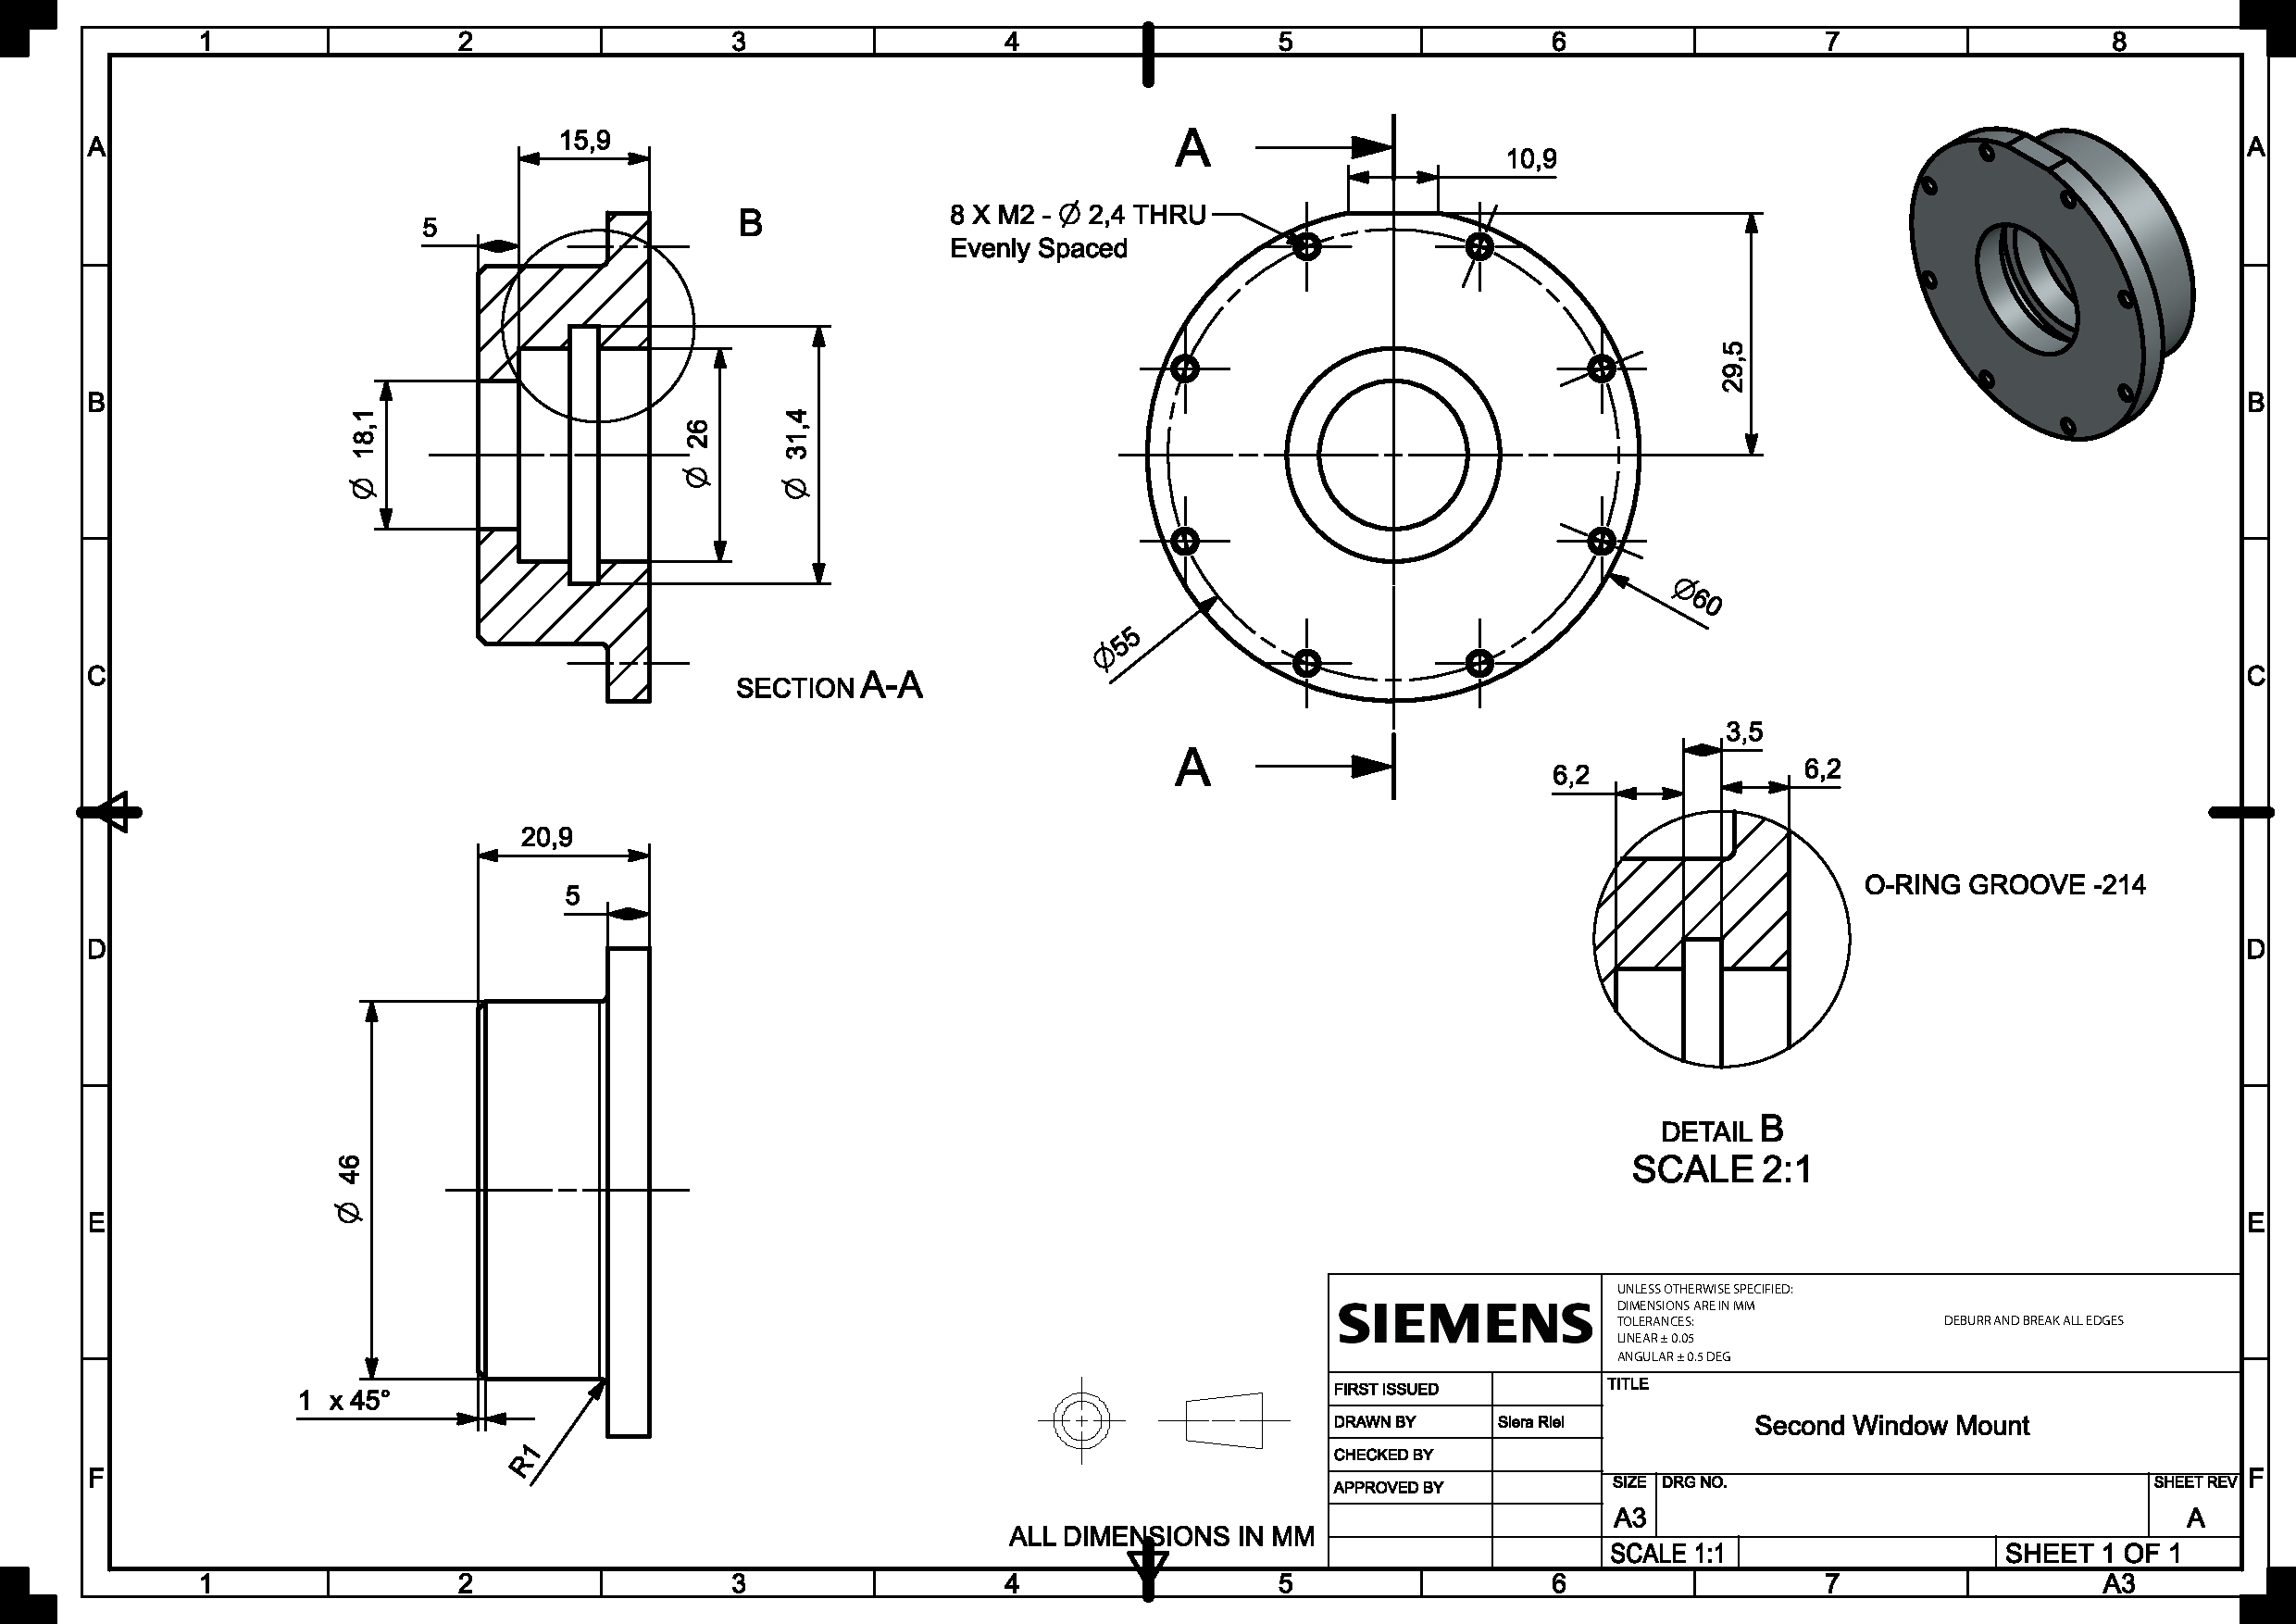
\includepdf[pages=-, pagecommand={\footeronly}]{assets/appendices/New V2 parts/Second Window Mount Final.pdf}
    \chapter{Untested V2 Parts Drawings}
        \includepdf[pages=-, pagecommand={\footeronly}]{assets/appendices/New V2 parts/sriel2_Extension cylinder real.pdf}\label{chp:Extension cylinder}
        \includepdf[pages=-, pagecommand={\footeronly}]{assets/appendices/New V2 parts/Inner Cylinder.pdf}\label{chp:remachined inner cylinder}
        \includepdf[pages=-, pagecommand={\footeronly}]{assets/appendices/New V2 parts/Exchangeable Nozzle.pdf}\label{chp:New nozzle}
        \includepdf[pages=-, pagecommand={\footeronly}]{assets/appendices/New V2 parts/sriel2_Exchangeable Nozzle Plate_inches.pdf}\label{chp:Exchangeable nozzle plate}
        \includepdf[pages=-, pagecommand={\footeronly}]{assets/appendices/New V2 parts/Higher Width Plate.pdf}\label{chp:thicker plate}

    % List of appendicies that I want:
        % [x] Laser and colimator calibration
        % [x] Bubble meter calibration Thariq's report
        % [x] Drawings for V2 from Capstone team
        % [x] V2 rear window mount
        % Drawings of untested parts
            % [x] Modified inner cylinder
            % [x] Spacer for static tests
            % [x] Flat plate with hole for bubble tests
            % [x] Flat plate for changeable graphite nozzles
            % [x] Graphite nozzles
    
\end{document}